\documentclass[11pt]{article}
\usepackage{array,booktabs,arydshln,xcolor}
\usepackage{tikz}
\usetikzlibrary{arrows}
\usetikzlibrary{patterns.meta}
\usetikzlibrary{decorations.pathreplacing}
\usetikzlibrary{decorations.markings,fpu}
\usetikzlibrary{decorations.pathmorphing}
\usepackage{amsmath}

\newcommand{\e}{\varepsilon}

\begin{document}

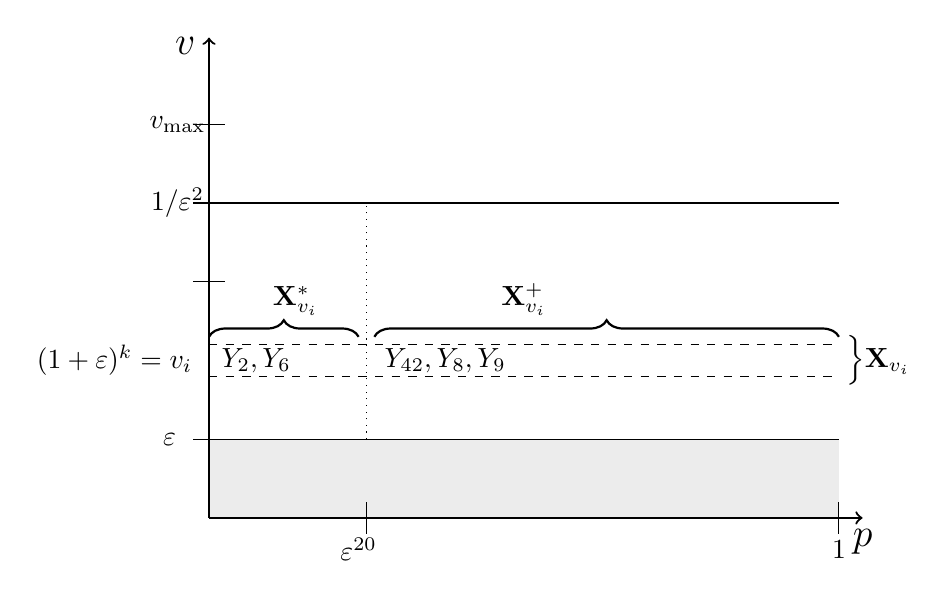
\begin{tikzpicture}

\pgfmathtruncatemacro{\casesL}{2};
\pgfmathtruncatemacro{\totalL}{8};
\pgfmathtruncatemacro{\vi}{2.5};

\tikzset{mycolor/.style={fill=gray!30, opacity=.5}}
%Fill shapes with color
\fill[mycolor] (0,0)--(0,1)--(\totalL,1)--(\totalL,0);

%Draw horizontal lines
\draw[->, thick] (0,0)--(0,\totalL-1.9) node[]{};
\draw[-] (0,1)--(\totalL,1) node[]{};
\draw[-] (0,4)--(\totalL,4) node[]{};

%Draw vertical lines
\draw[-, dotted] (\casesL,1)--(\casesL,4) node[]{};
\draw[->, thick] (0,0)--(\totalL+0.3,0) node[]{};

%y axis labels
\node[] at (-0.4,5) {$v_{\max}$};
\draw[-] (-0.2, 5) --(0.2,5);
\node[] at (-0.4,4) {$1/\e^2$};
\draw[-] (-0.2, 4) --(0.2,4);
\draw[-] (-0.2, 3) -- (0.2, 3);
\node[] at (-1.2,\vi) {$(1+\e)^k=v_i$};
\node[] at (-0.5,1) {$\e$};
\draw[-] (-0.2, 1) --(0.2,1);

%Draw box with variables
\draw[-, dashed] (0,\vi-0.2)--(\totalL,\vi-0.2) node[]{};
\draw[-, dashed] (0,\vi+0.2)--(\totalL,\vi+0.2) node[]{};
\node[] at (0.6,\vi) {$Y_{2}, Y_6$};
\node[] at (\casesL+1,\vi) {$Y_{42}, Y_8, Y_9$};
\node[] at (\totalL+0.5,\vi) {${ \Big \} } \mathbf{X}_{v_i}$};

%Legend on axes
\node[] at (-0.3,\totalL-2) {{\Large $v$}};
\node[] at (\totalL+0.3,-0.3) {{\Large $p$}};
	
%x axis labels
\node[] at (\casesL-0.1,-0.4) {$\e^{20}$};
\draw[-] (\casesL, -0.2) -- (\casesL, 0.2);
\draw[-] (\totalL, -0.2) -- (\totalL, 0.2);
\node[] at (\totalL, -0.4) {$1$};

%Draw braces + labels
\draw [decorate,black,thick,decoration={brace,amplitude=6pt}] (0,\vi+0.3) -- (\casesL-0.1,\vi+0.3) node[label={[xshift=-0.8cm, yshift=0.01cm]$\mathbf{X}^*_{v_i}$}]{};

\draw [decorate,black,thick,decoration={brace,amplitude=6pt}] (\casesL+0.1,\vi+0.3) -- (\totalL,\vi+0.3) node[label={[xshift=-4cm, yshift=0.01cm]$\mathbf{X}^+_{v_i}$}]{};

\end{tikzpicture}

\end{document}